\chapter{Juegos de Rol}
\label{cap:juegosrol}

\begin{resumen}
En este capítulo se explicará qué son los juegos de rol, se introducirá su historia, y se examinarán algunos de los juegos de rol más importantes.
\end{resumen}

\section{¿Qué es un juego de rol?}
Los juegos de rol (RPG, \textit{role-playing game}) son, en palabras de \citeauthor{LortzRPG} (\citeyear{LortzRPG}, como se cita en \cite{FineRPG}), \comillas{todos aquellos juegos que permiten a un determinado número de jugadores asumir los roles de personajes imaginarios y operar con cierto grado de libertad en un entorno imaginario}. 

\medskip

Este tipo de juegos se caracteriza por una base muy sólida, que \cite{TychsenRPG} resumen en los siguientes elementos:

\begin{itemize}
	\item \textbf{Narrativa estructurada por reglas}: los juegos de rol se basan en contar una historia dentro de un marco de reglas específicas. Tanto la narrativa como las reglas son únicas para cada juego, proporcionando una estructura que guía la progresión de este y las decisiones de los jugadores.
	\item \textbf{Participación múltiple y mundo ficticio compartido}: los juegos de rol requieren de la participación de múltiples jugadores (al menos dos), quienes interactúan dentro de un mundo ficticio común. Es esencial que todos los participantes comprendan la ambientación, el entorno y las reglas antes de comenzar la partida.
	\item \textbf{Control de personajes por parte de los jugadores}: la mayoría de los participantes asumen el control de al menos un personaje durante toda la partida. A través de estos personajes, los jugadores interactúan con el entorno y con otros personajes, desarrollando la narrativa del juego.
	\item \textbf{Dirección del juego mediante un instructor}: por lo general, existe la figura del director de juego (GM, \textit{gamemaster}) que administra los aspectos del juego no controlados directamente por los jugadores. El \textit{gamemaster} facilita el flujo del juego, proporciona contenido ambiental del mundo ficticio y arbitra las reglas y los conflictos que puedan surgir.
\end{itemize}

\medskip

Sumado a estos elementos estructurales, se encuentran otras características igualmente esenciales para definir la experiencia de un juego de rol:
\begin{itemize}
	\item \textbf{Progresión del personaje}: los personajes evolucionan mecánica, narrativa y emocionalmente a lo largo del tiempo mediante la obtención de puntos de experiencia que se pueden \comillas{gastar} en un sistema de niveles \citep{barton2008dungeons}.
	\item \textbf{Inmersión}: resulta fundamental para comprender el atractivo de este género, permitiendo a los jugadores experimentar emociones y tomar decisiones desde la perspectiva de sus personajes \citep{Montola2010}.
	\item \textbf{Narrativa emergente}: es decir, la construcción dinámica y colaborativa de la historia a partir de las acciones de los participantes \citep{FineRPG}.
 	\item \textbf{Decisiones significativas}: las decisiones de los jugadores deben tener consecuencias reales en el desarrollo de la partida \citep{tekinbas2003rules}.
	\item \textbf{Alto grado de flexibilidad y adaptabilidad}: las reglas, ambientaciones o mecánicas se pueden modificar dependiendo de las necesidades del grupo, lo que evidencia un carácter modular y abierto \citep{Edwards2001}.
\end{itemize} 

\medskip

Por otra parte, existen algunos aspectos menos formalizados pero igualmente importantes para el funcionamiento y disfrute de los juegos de rol, como por ejemplo, un contrato social, en el que los jugadores acuerden las temáticas permitidas, el tono de la partida y las dinámicas sociales; una coherencia tonal y de género, que permita mantener una ambientación y tonos coherentes para la inmersión en la partida; fomento de la expresividad de los jugadores, es decir, beneficiarse del uso de la voz, gestos y una narración detallada para enriquecer la interpretación de los personajes; libertad de improvisación frente a lo inesperado; y la exploración emocional y empática con realidades ajenas.

\medskip

En conjunto, todos estos elementos conforman una experiencia lúdica rica, dinámica y profundamente humana, donde la colaboración, interpretación y narrativa se entrelazan de forma única. Lejos de limitarse a un solo modelo, los juegos de rol han dado lugar a una amplia variedad de formas y enfoques, cada uno con sus propias mecánicas, estilos narrativos y niveles de complejidad.

\subsection{Tipos de juegos de rol}
A lo largo del tiempo, los juegos de rol han evolucionado en múltiples direcciones, dando lugar a distintas topologías con enfoques, estructuras y estilos de juego muy variados. Atendiendo a estas características, se presenta una clasificación general de los tipos más representativos:

\subsubsection{Juegos de rol de mesa o tablero}
Los juegos de rol de mesa (TTRPG, \textit{tabletop role-playing games}), constituyen la forma más tradicional de juegos de rol. En este tipo de juegos, los jugadores se reúnen en torno a una mesa física o virtual y cada uno asume el papel de un personaje ficticio. Uno de los participantes actúa como GM, responsable de narrar la historia, interpretar a los NPC (\textit{non-player character}, personaje no jugador) y arbitrar las reglas.

\medskip

Uno de los elementos más representativos de los TTRPG es el uso de dados poliédricos para resolver acciones inciertas. Por ejemplo, en \cite{ogdnd}, se utiliza un dado de veinte caras (popularmente conocido como \comillas{d20}) para realizar la mayoría de las pruebas. Si un personaje intenta realizar una acción desafiante, como escalar una pared o atacar a un enemigo, el jugador tira el dado y suma ciertos modificadores; si el resultado iguala o supera una dificultad determinada por el GM, la acción tendrá éxito.

\medskip

Estos juegos también incluyen hojas de personaje con estadísticas numéricas (como fuerza, inteligencia o destreza), inventarios, puntos de vida y habilidades especiales. Además, el progreso de los personajes se da mediante la adquisición de experiencia, lo que permite mejorar atributos, aprender nuevas habilidades o subir de nivel.

\subsubsection{Juegos de rol en vivo}
\figura{Bitmap/nordiclarp}{width=0.9\textwidth}{fig:nordiclarp}{Partida de LARP nórdico, extraída de \cite{nordiclarpimg}.}

Los juegos de rol en vivo (LARP, \textit{live-action role-playing game}) son una variante en la que los participantes interpretan físicamente a sus personajes en un espacio real, vistiéndose y actuando conforme a su rol. No se juega en torno a una mesa, sino que se representa la historia a través de la acción directa, muchas veces con elementos de escenografía, vestuario y una mayor carga teatral.

\medskip

Las reglas suelen ser simplificadas o adaptadas para no interrumpir el flujo de la interpretación, y en muchos casos se utilizan sistemas de señales o puntos para resolver conflictos, en lugar de dados. En ciertos LARP de combate, se emplean armas acolchadas para simular enfrentamientos físicos.

\medskip

Este formato se presta especialmente para la exploración emocional, la inmersión profunda y la representación de tramas políticas, sociales o dramáticas.

\medskip

Dentro del género LARP, encontramos el subgénero de LARP nórdico, inspirado en la cultura nórdica en la que el fracaso es parte de la trama y es mucho más artístico que los LARP tradicionales, como se puede apreciar en la figura \ref{fig:nordiclarp}, con la recreación de un dragón a tamaño real y el involucramiento de numerosos jugadores.

\subsubsection{Juegos de rol por foro o texto}
Este tipo de juegos se desarrollan completamente por escrito, ya sea en foros de internet, chats o correos electrónicos. Los participantes escriben mensajes en los que narran las acciones, pensamientos y diálogos de sus personajes, construyendo la historia de manera colaborativa.

\medskip

A menudo carecen de un sistema rígido de reglas o tiradas de dados, y dependen más de la narración consensuada y de la calidad interpretativa. En algunos casos se incorporan sistemas de puntos, turnos o moderados para mantener la coherencia y el equilibrio del juego.

\medskip

Este tipo de juego permite un desarrollo más introspectivo de los personajes y tramas más complejas, ya que los jugadores disponen de tiempo para redactar sus intervenciones.

\subsubsection{Juegos de rol digitales}
Los juegos de rol digitales (CRPG, \textit{computer role-playing games}, juegos de rol de ordenador) son videojuegos que adoptan las mecánicas y estructuras de los juegos de rol tradicionales.

\medskip

Sobre este tema se ampliará más en el capítulo \ref{cap:videojuegosrol}, donde se tratará en profundidad todo lo relacionado con este género de videojuegos.

\subsubsection{Comparativa}
A modo de resumen, se incluye una tabla comparativa entre los distintos tipos anteriormente vistos.
\begin{table}[H]
	\centering
	\scalebox{0.85}{
	\begin{tabular}{c|c|c|c} 
		\textbf{Tipo de juego} & \textbf{Medio} & \textbf{Resolución de acciones} & \textbf{Nivel de inmersión} \\
		\hline\hline 
		Rol de mesa (TTRPG) & Presencial / Virtual & Dados y reglas estructuradas & Alto \\
		Rol en vivo (LARP) & Presencial & Señales, puntos o actuación directa & Alto \\
		Rol por foro / texto & Digital (escrito) & Narración compartida y consenso & Alto \\					Rol digital (CRPG) & Videojuegos & Algoritmos computacionales & Variable \\
		\hline
	\end{tabular}
	}
\end{table}

\section{Historia de los juegos de rol}

La historia de los juegos de rol está íntimamente ligada a la evolución de los juegos de estrategia, la literatura de fantasía y la experimentación lúdica del siglo XX. Su origen puede rastrearse a las décadas de 1960 y 1970, con influencias que abarcan desde los \textit{wargames} (juegos de guerra) hasta las obras de J.R.R. Tolkien.

\medskip

\figura{Bitmap/kriegsspiel}{width=0.7\textwidth}{fig:kriegsspiel}{Tablero de juego moderno de \cite{kriegsspiel}, extraída de \cite{kriegsspielimg}.}

Los juegos de rol tienen sus raíces en los \textit{wargames}, juegos de estrategia militar que simulan conflictos bélicos con miniaturas y mapas. Entre ellos se destaca el pionero \cite{kriegsspiel}, diseñado por un noble prusiano que quería dotar al ejército de un entrenamiento táctico en caso de guerra. En la figura \ref{fig:kriegsspiel} podemos ver el tablero de juego, consistente en una representación cartográfica de un territorio real, y, encima, las unidades militares de ambos bandos (cada una de un color, y cada rango dependiendo del patrón dibujado).

\smallskip

Este tipo de juegos de mesa se fueron desarrollando con el paso del tiempo, apareciendo también libros que contenían una serie de reglas para desarrollar partidas más interesantes, como es el caso de \textit{Little Wars} \citep{littlewars}, convirtiendo a este tipo de juegos en simulaciones mucho más narrativas.

\medskip

No es hasta la década de los 70, con la aparición de juegos como \cite{chainmail}, que la comunidad comienza a incorporar elementos de personajes individuales y no colecciones de unidades militares. Con este suceso, se comienza a hablar propiamente de \comillas{juegos de rol}, y se empiezan a ver los primeros juegos comerciales de este tipo.

\medskip

Se considera que \cite{ogdnd} es el primer juego de rol comercial. Este juego combinaba reglas derivadas de los \textit{wargames} con elementos narrativos inspirados en la literatura fantástica. Cada jugador asumía el papel de un aventurero (por ejemplo, un guerrero o un mago) y exploraba mazmorras, resolvía acertijos y combatía monstruos, todo bajo la guía de un GM. Esta revolucionaria idea de interpretar un personaje y tomar las decisiones desde su perspectiva sentó las bases de este género, que poco a poco se fue popularizando.

\medskip

En la década de los 80, este género se expandió, dando a lugar a nuevos sistemas y ambientaciones, como la saga de horror \cite{cthulhu} o la de fantasía \cite{rq}. Los temas y las mecánicas comienzan a diversificarse, y se comienzan a publicar suplementos, novelas y productos derivados que expandían los universos de los juegos. También aparecen los primeros videojuegos que incorporaban mecánicas de estos juegos de tablero, apareciendo el género de los CRPG. Es a finales de esta época cuando comienzan a surgir los primeros LARP, y se empiezan a organizar convenciones temáticas, consolidando la cultura de jugadores de este género.

\medskip

Entrando en la nueva década, crecen las comunidades LARP tanto en Estados Unidos como en Europa gracias a juegos como \cite{mindseye}, mientras que la normalización de internet en los hogares permitió el surgimiento del rol por foro y correo electrónico, ampliando el acceso a este tipo de contenidos.

\medskip

Finalmente, en el siglo XXI, el rol se diversificó aún más. Los CRPG se volvieron cada vez más complejos y tenían un mayor alcance, surgen los MMORPG (\textit{massively multiplayer online role-playing game}, videojuegos de rol multijugador masivos en línea), que ofrecen experiencias compartidas masivas, mientras que el auge de plataformas como Discord, Roll20 o Foundry Virtual Tabletop revitalizó el juego de rol de mesa en línea.

\medskip

La popularización del \textit{streaming} en la década del 2010, y la aparición de \textit{podcasts} de rol como \textit{Critical Role} ayudaron a introducir el género a nuevas generaciones, mostrando su gran potencial narrativo y creativo. Hoy en día, los juegos de rol son practicados por millones de personas en todo el mundo, en formatos que van desde campañas caseras hasta multitudinarios eventos de LARP, o desde videojuegos AAA hasta partidas por texto en móviles.

\section{Análisis de los principales juegos de rol}

\subsection{\textit{Dungeons \& Dragons}}
\begin{figure}[t]
\centering
\begin{SubFloat}
{\label{fig:dndsencillo}%
	Imagen de una partida común de D\&D, extraída de \cite{dndsencillaimg}.}%
	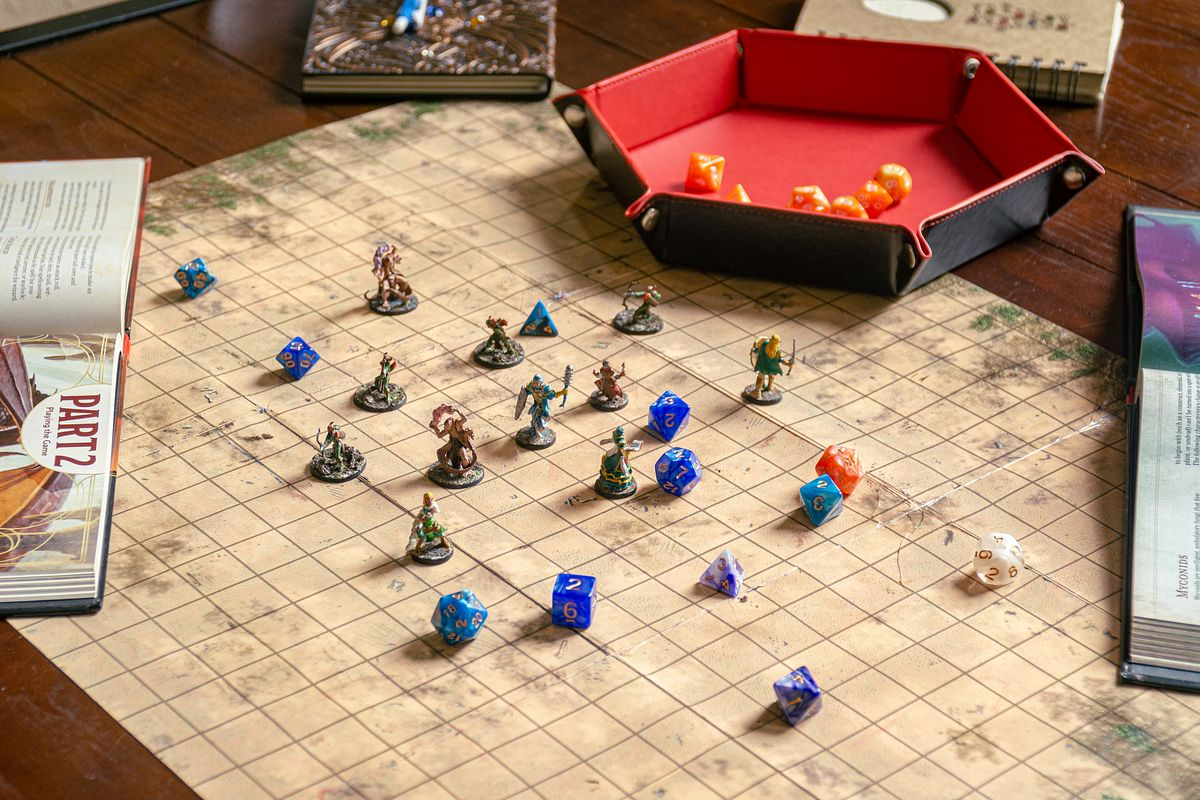
\includegraphics[width=0.45\textwidth]{Imagenes/Bitmap/dndsencillo}%
\end{SubFloat}
\qquad
\begin{SubFloat}
{\label{fig:dnddiorama}%
	Imagen de un diorama para el escenario de una partida de D\&D, extraída de \cite{dnddioramaimg}.}%
	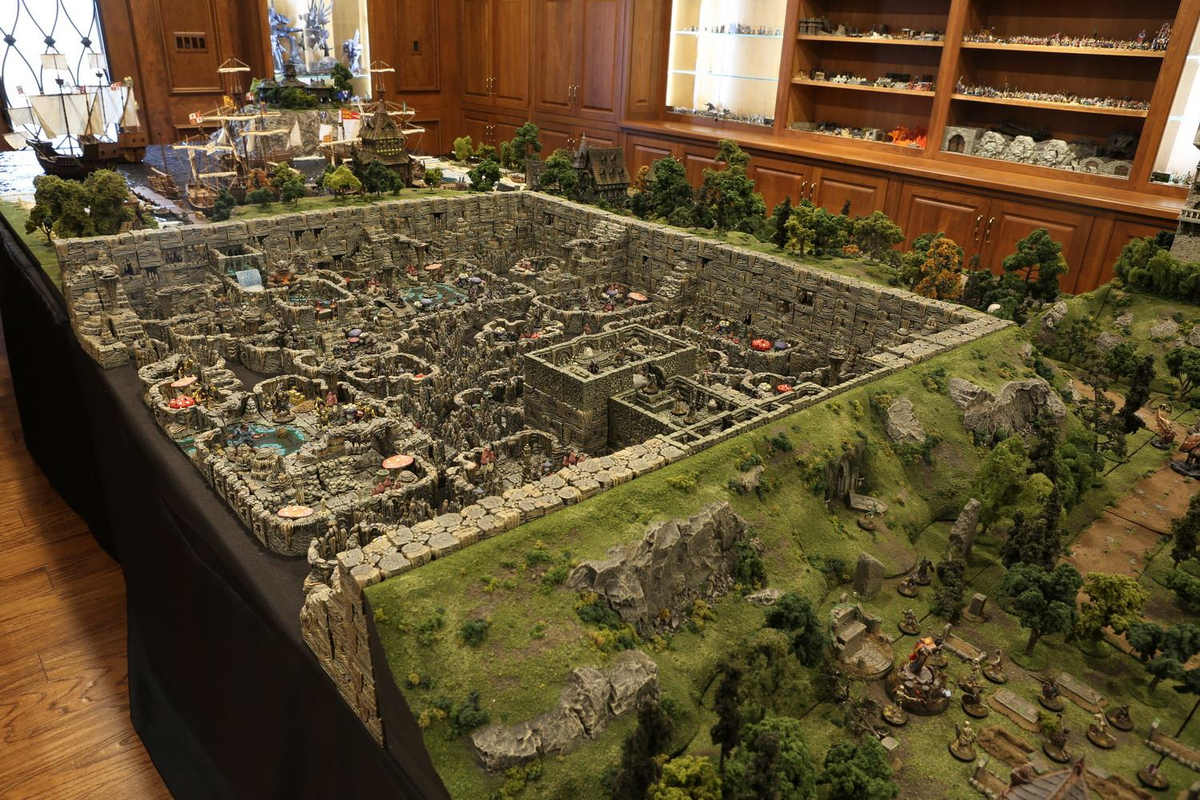
\includegraphics[width=0.45\textwidth]{Imagenes/Bitmap/dnddiorama}%
\end{SubFloat}
\caption{Imágenes de distintas variedades de partidas de \textit{Dungeons \& Dragons}. \label{fig:dndejemplos}}
\end{figure}

Como se ha mencionado anteriormente, \cite{ogdnd}, a veces conocido únicamente como D\&D, es ampliamente conocido como el primer juego de rol comercial y el más influyente del género, y su origen se basa en el sistema de reglas de \cite{chainmail}, al cual se le añadieron elementos de exploración, personajes individuales y narrativa.

\medskip

D\&D se estructura en torno al concepto de un grupo de aventureros que exploran mundos de fantasía, enfrentan criaturas, resuelven conflictos y evolucionan mediante un sistema de niveles y experiencia. El director de juego (aquí llamado \textit{dungeon master}, DM) narra la historia, describe el mundo y controla a los NPC y eventos.

\smallskip

A partir de la tercera edición, del año 2000, se introduce el \textit{sistema d20}, un dado de veinte caras en el que se basa todo el sistema de reglas, así como hojas de personaje detalladas con diversos atributos.

\medskip

En la figura \ref{fig:dndejemplos} podemos ver varios ejemplos de partidas de D\&D, siendo la que está capturada en la figura \ref{fig:dndsencillo} un ejemplo de una partida normal, con un tablero y sus diferentes \textit{d20}, y, en la figura, \ref{fig:dnddiorama}, un ejemplo de un diorama creado por un aficionado a la maquetación, que cuenta con todo lujo de detalles y que llega a ocupar toda una sala.

\medskip

El juego ha pasado por múltiples ediciones, cada una introduciendo cambios en las mecánicas, balance y filosofía de diseño. Su edición más reciente, la quinta, del año 2014, ha tenido un gran éxito comercial y ha contribuido al resurgimiento del juego de rol gracias a su gran accesibilidad, su enfoque narrativo y la visibilidad en plataformas como YouTube o Twitch.

\medskip

El impacto de este juego en la cultura popular y en el diseño de otros juegos es difícil de sobreestimar, ya que está considerado el estándar de facto en los TTRPG y ha inspirado hasta adaptaciones cinematográficas\footnote{La saga \textit{Dungeons \& Dragons} \citep{dndpeli} ha recaudado más de 250 millones de dólares en total sumando las cuatro películas, siendo la última entrega, de 2023, la más exitosa de todas.}.

\subsection{\textit{Pathfinder}}
\cite{pathfinder} nació como una evolución del \textit{sistema d20} de D\&D. Ante el cambio de enfoque que supuso la cuarta edición de D\&D, muchos jugadores buscaron una alternativa que conservara la complejidad y flexibilidad del sistema anterior. Se aprovechó de la licencia OGL (\textit{Open Game License}, Licencia de Juego Abierto)\footnote{Esta licencia se usa principalmente en TTRPG y concede, por parte de los diseñadores, permisos de modificación, copia y redistribución de algunos de los contenidos diseñados para sus juegos, principalmente mecánicas.} para crear un sistema propio que mejorara y expandiera el marco de reglas original.

\medskip

El juego destaca por su nivel de detalle, la personalización de personajes y la riqueza de opciones tácticas durante el combate. El sistema de creación de personajes permite una gran variedad de combinaciones de clases, habilidades, dotes y objetos mágicos. Esto atrae especialmente a jugadores que valoran la optimización mecánica y la profundidad estratégica.

\medskip

Narrativamente, matiene el enfoque épico y de alta fantasía de D\&D, pero con mundos propios, combinando elementos clásicos con tramas políticas, horror cósmico o mitologías exóticas.

\smallskip

En 2019 se publicó su segunda edición, que renovó el sistema con nuevas mecánicas más modernas, como un sistema de tres acciones por turno y una progresión más clara. Pese a que no ha alcanzado el nivel de popularidad de D\&D, \textit{Pathfinder} ha consolidado una gran comunidad y ha mantenido una identidad propia, por lo que muchas páginas lo sitúan siempre en segundo o tercer lugar de popularidad\footnote{La página \textit{The Dragon's Trove} lo sitúa en tercer lugar en su histórico: \url{https://www.dragonstrove.com/blogs/news/the-best-tabletop-rpgs-of-all-time}.}.

\subsection{\textit{Call of Cthulhu}}
\cite{cthulhu} está basado en los mitos creados por H.P. Lovecraft, y representa un enfoque radicalmente distinto al de otros juegos de rol de la época, ya que se centra en la investigación, el horror psicológico y la fragilidad humana ante lo desconocido.

\medskip

El sistema utiliza como base las reglas BRP {\textit{Basic Role-Playing}, Juego de Rol Básico}, que utiliza porcentajes para determinar el éxito de las acciones. Los personajes son investigadores en los años 20 (aunque hay adaptaciones a otras épocas), y deben enfrentarse a cultos secretos, criaturas indescriptibles y horrores cósmicos. A diferencia de otros juegos, la muerte o locura de los personajes es común y está integrada en la narrativa, lo que fomenta una experiencia inmersiva y tensa.

\medskip

El atributo de cordura (SAN, del inglés \textit{sanity}) es central, ya que los encuentros con lo sobrenatural pueden erosionar la mente de los personajes hasta conducirlos a la locura. Esta mecánica refleja la atmósfera opresiva de las obras \textit{lovecraftianas} y crea un estilo de juego más introspectivo y sombrío.

\medskip

\textit{Call of Cthulhu} ha sido aclamado por su capacidad de generar tensión narrativa, y ha influido en muchos otros juegos de rol e investigación, convirtiéndolo en un pilar fundamental del rol narrativo.

\subsection{\textit{Warhammer Fantasy Roleplay}}
\figura{Bitmap/warhammer}{width=0.9\textwidth}{fig:warhammer}{Partida de \textit{Warhammer Fantasy Battle}, extraída de \cite{warhammerimg}.}

\cite{warhammer} comparte ambientación con el universo de miniaturas de \cite{warhammerbattle} (ver figura \ref{fig:warhammer}), pero se diferencia por su tono más oscuro, realista y decadente.

\medskip

Ambientado en un mundo inspirado en la Europa del Renacimiento, pero plagado de corrupción, magia caótica y criaturas monstruosas, WFRP pone al jugador en la piel de personajes que suelen comenzar como personas comunes (rateros, campesinos o aprendices), y no como héroes épicos. El juego enfatiza la progresión lenta, la supervivencia y la toma de decisiones difíciles.

\medskip

Su sistema de reglas, basado también en porcentajes, incluye un sistema de carreras profesionales que estructura el desarrollo del personaje de forma naturalista. Las heridas son graves, la corrupción mágica puede deformar al personaje, y la muerte puede llegar de forma repentina. Esto genera un entorno de juego más peligroso y centrado en la narrativa emergente.

\medskip

WFRP es un referente del estilo conocido como \textit{grimdark}\footnote{La expresión \textit{grimdark} proviene de una de las entregas de la saga \textit{Warhammer}, concretamente, \textit{Warhammer 40000}, en la que se explica que \comillas{In the \textbf{grim dark}ness of the far future there is only war} (En la sombría oscuridad del futuro lejano solo hay guerra).}, que enfatiza mundos crueles, moralidades grises y destinos trágicos. Esta saga ha sido particularmente influyente en Europa, y ha servido de inspiración para sagas de videojuegos como la de \textit{The Witcher}.